% ==============================================================================
%  データサイエンス 第一回講義課題：履修者アンケートの定量的分析
%  72603857_鈴木真理_1.tex (uplatex + dvipdfmx) — A4 × 3 pages
% ==============================================================================
\documentclass[uplatex, dvipdfmx, a4paper, 10pt]{jsarticle}

\usepackage[top=15truemm,bottom=15truemm,left=18truemm,right=18truemm]{geometry}
\usepackage{amsmath, amssymb, mathtools, bm}
\usepackage[dvipdfmx]{graphicx}
\usepackage{float}
\usepackage{booktabs}
\usepackage{caption}
\usepackage[dvipdfmx, bookmarks=true, setpagesize=false, colorlinks=true, linkcolor=black, urlcolor=blue, citecolor=black]{hyperref}
\usepackage{pxjahyper}
\usepackage{listings}
\usepackage{xcolor}
\usepackage{tabularx}
\usepackage{enumitem}
\usepackage{multicol}

\definecolor{codegreen}{rgb}{0,0.6,0}
\definecolor{codegray}{rgb}{0.5,0.5,0.5}
\definecolor{codepurple}{rgb}{0.58,0,0.82}
\definecolor{backcolour}{rgb}{0.95,0.95,0.92}
\lstdefinestyle{mystyle}{
    backgroundcolor=\color{backcolour},
    commentstyle=\color{codegreen},
    keywordstyle=\color{magenta},
    numberstyle=\tiny\color{codegray},
    stringstyle=\color{codepurple},
    basicstyle=\ttfamily\scriptsize,
    breakatwhitespace=false, breaklines=true,
    captionpos=b, keepspaces=true,
    numbers=left, numbersep=4pt,
    showspaces=false, showstringspaces=false, showtabs=false,
    tabsize=2, frame=single,
    aboveskip=3pt, belowskip=1pt
}
\lstset{style=mystyle}

% --- Macros ---
\newcommand{\ns}{\textrm{\scriptsize n.s.}}

% --- Aggressive Spacing ---
\setlength{\parskip}{0.5pt plus 0.3pt}
\setlength{\abovecaptionskip}{2pt}
\setlength{\belowcaptionskip}{0pt}
\setlength{\floatsep}{2pt plus 1pt minus 1pt}
\setlength{\textfloatsep}{3pt plus 1pt minus 1pt}
\setlength{\intextsep}{2pt plus 1pt minus 1pt}
\setlist{nosep, leftmargin=1.5em, topsep=0pt, partopsep=0pt}
\captionsetup{font=small, skip=1pt}

% --- Reduce section/subsection spacing ---
\makeatletter
\renewcommand{\section}{\@startsection{section}{1}{\z@}%
  {0.5\Cvs \@plus.15\Cvs \@minus.05\Cvs}%
  {0.1\Cvs \@plus.05\Cvs}%
  {\normalfont\large\headfont\raggedright}}
\renewcommand{\subsection}{\@startsection{subsection}{2}{\z@}%
  {0.3\Cvs \@plus.1\Cvs \@minus.05\Cvs}%
  {0.05\Cvs \@plus.03\Cvs}%
  {\normalfont\normalsize\headfont\raggedright}}
\makeatother

% ==============================================================================
\title{\vspace{-10mm}データサイエンス 第一回講義課題\\ \normalsize 履修者アンケートの定量的分析 By 鈴木真理\vspace{2mm}\\ \normalsize 履修者アンケートの定量分析By Gemini\vspace{2mm}}
\author{\small 慶應義塾大学 総合政策学部\quad 学籍番号: 72603857\quad 鈴木 真理}
\date{\small \today}

\begin{document}
\maketitle
\vspace{-7mm}

% ====================== PAGE 1: Overview & Macro Statistics ===================
\begin{abstract}\small\setlength{\parskip}{0pt}
    本レポートでは，2026年度春学期データサイエンス講義の履修者912名のスキルアンケートを定量的に分析した．
    核心は3点に集約される：
    \textbf{(1)} Python・SQL・R間に有意な正の相関，特にPython$\times$SQLが最強（$r\!=\!0.450$, $p\!<\!0.0001$）；
    \textbf{(2)} 学部間差はPython・他PGのみ限定的に有意；
    \textbf{(3)} 性別間ではPG系で男性が有意に高く，Gender Neutrality仮説は棄却．
\end{abstract}

\vspace{-1mm}
\section{はじめに}

データサイエンス教育の効果的設計には，履修者の事前スキル分布の把握が不可欠である．
本レポートでは，慶應義塾大学SFCの2026年度春学期データサイエンス講義・第1回アンケート
（$N\!=\!912$; 環境情報508, 総合政策385, 他19; 男629, 女279）を対象に3つの仮説を検証する：
\textbf{H1.}~Python・R・SQL間に正の相関あり．
\textbf{H2.}~学部間にスキル差あり．
\textbf{H3.}~性別による偏りなし（Gender Neutrality）．
全カラムで欠損0件，表記揺れ（計28件）を対処済み．

\vspace{1mm}
\noindent
\begin{minipage}[t]{0.52\linewidth}
    \subsection{基本統計量（Descriptive Statistics）}
    \vspace{-2mm}
    \begin{table}[H]
        \centering\small
        \caption{スキル別基本統計量}
        \label{tab:basic_stats}
        \begin{tabular}{@{}lccc@{}}
            \toprule
            \textbf{スキル}    & \textbf{Mean} & \textbf{SD}   & \textbf{Med.} \\
            \midrule
            Excel分析         & 2.16          & 0.80          & 2             \\
            Pivot Table     & 1.54          & 0.73          & 1             \\
            SQL             & 1.34          & 0.68          & 1             \\
            R               & 1.58          & 0.73          & 1             \\
            \textbf{Python} & \textbf{2.22} & \textbf{0.77} & \textbf{2}    \\
            他PG             & 1.75          & 0.89          & 2             \\
            \bottomrule
        \end{tabular}
    \end{table}
\end{minipage}%
\hfill
\begin{minipage}[t]{0.46\linewidth}
    \vspace{2mm}
    \centering
    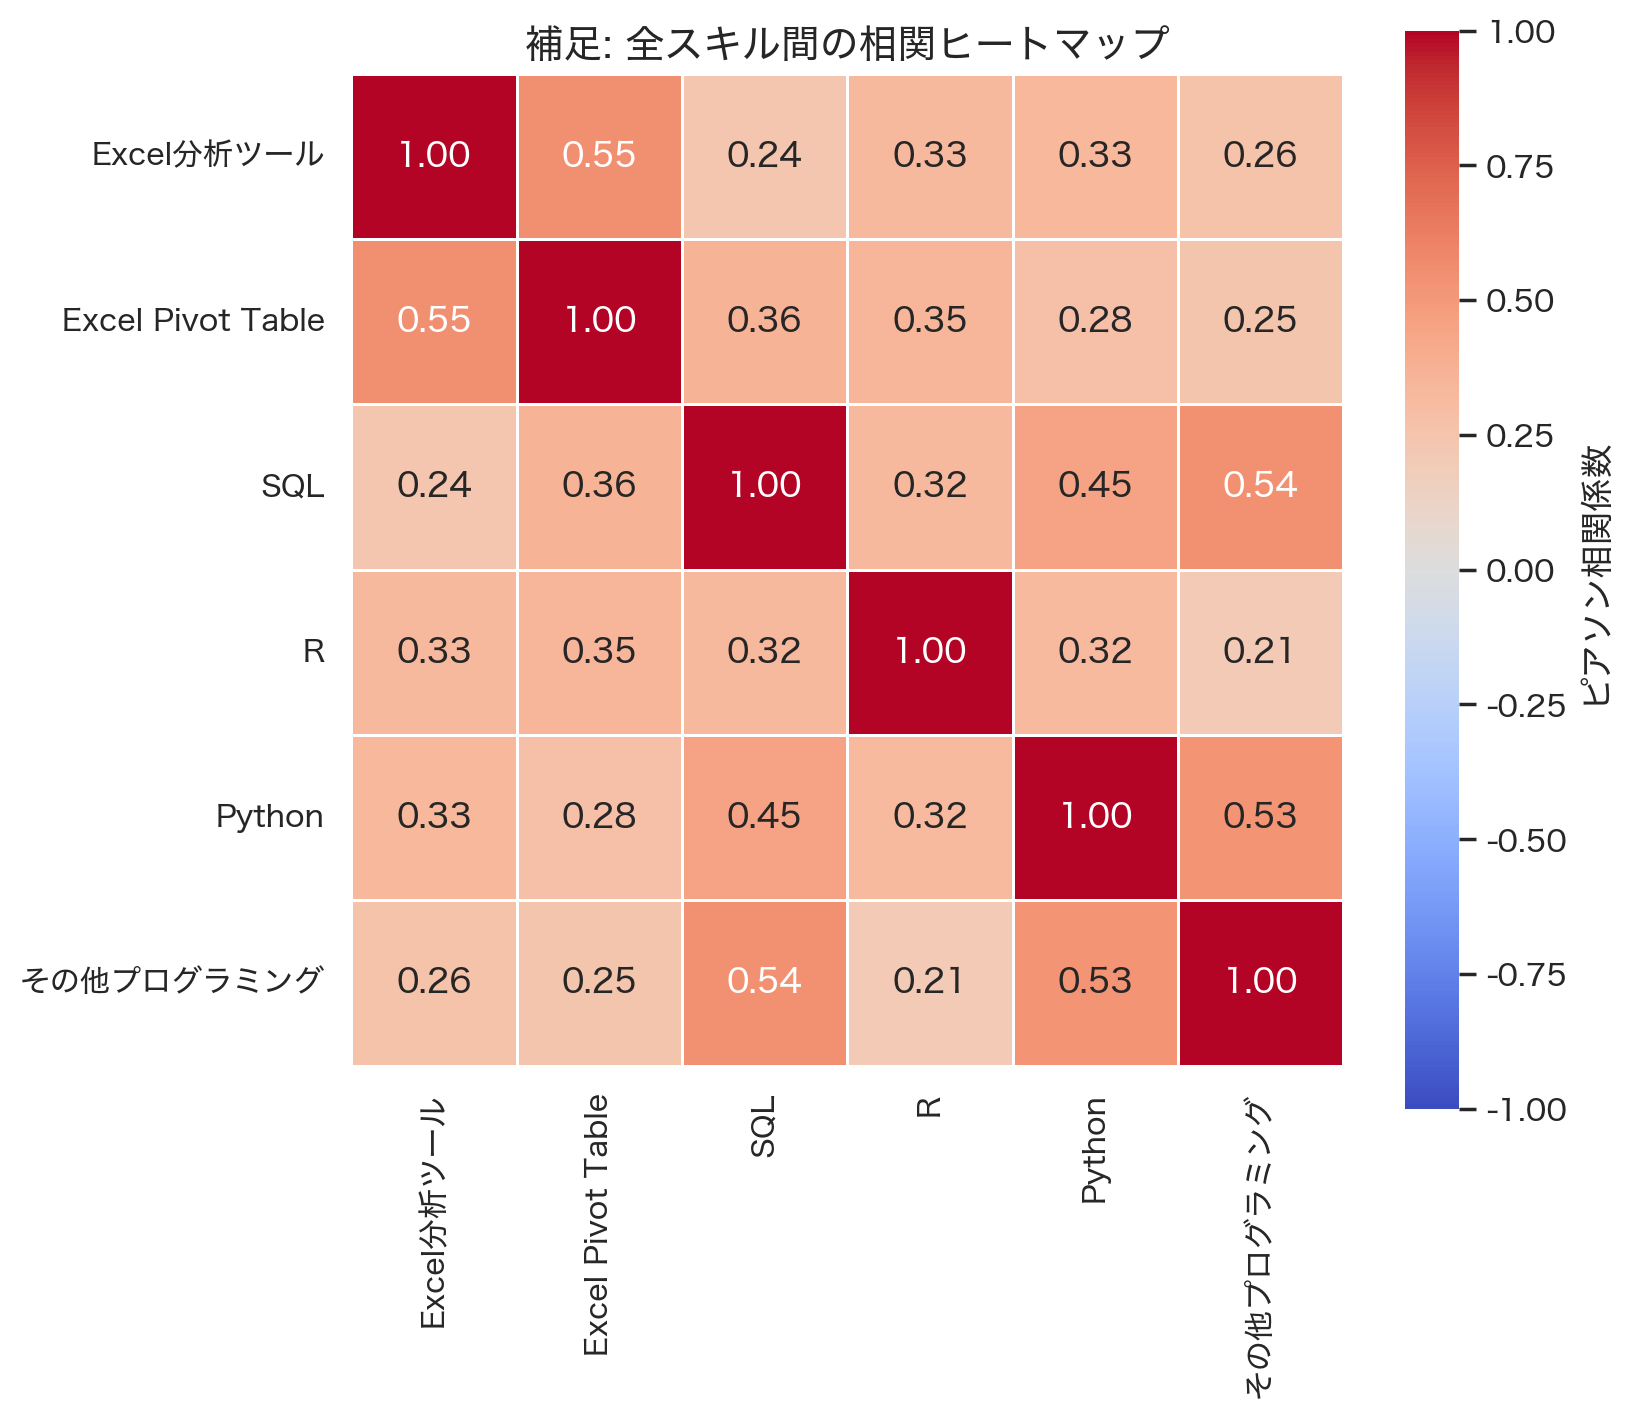
\includegraphics[width=\linewidth]{../Assets/h1_full_correlation_heatmap.png}
    \captionof{figure}{全スキル相関行列}
    \label{fig:full_heatmap}
\end{minipage}

\vspace{1mm}
Pythonが最高の平均値（$\bar{x}\!=\!2.22$）を示す一方，SQL・R・Pivotは中央値1（未経験）．
典型的な学生像は\textbf{「Python初心者〜中級者，他ツールは未経験」}と特徴づけられる．
図\ref{fig:full_heatmap}に示す相関行列から，「Excel系」と「PG系（Python/SQL/他）」の\textbf{2独立クラスター}が確認された．

% =========== PAGE 2: Hypothesis Testing & Quantitative Analysis ===============
\newpage
\section{仮説検証（Hypothesis Testing）}

\subsection{手法選択の根拠（Methodology）}

スキルデータは5段階順序尺度であり正規分布の仮定が困難なため，
2群比較にはノンパラメトリックなMann--Whitney $U$検定\cite{mann1947}を採用（正規性・等分散性不要，各群$n\!>\!279$）．
相関にはPearsonの積率相関係数\cite{pearson1895}を用いた．
順序尺度へのPearson $r$適用は，サンプルサイズが十分大きい場合に頑健な推定値を与えることが知られている．
有意水準$\alpha\!=\!0.05$，$^*p\!<\!.05$, $^{**}p\!<\!.01$, $^{***}p\!<\!.001$ 表記．

\subsection{H1: Python・R・SQL間の相関 --- \textmd{支持}}

\vspace{-1mm}
\begin{table}[H]
    \centering\small
    \caption{H1: ペアワイズ相関（Pearson $r$）}
    \label{tab:h1_corr}
    \begin{tabular}{@{}lcc c@{}}
        \toprule
        \textbf{ペア}                & \textbf{$r$}   & \textbf{$p$}       &                \\
        \midrule
        Python$\times$R            & 0.320          & $<$0.0001          & $***$          \\
        \textbf{Python$\times$SQL} & \textbf{0.450} & $<$\textbf{0.0001} & $\mathbf{***}$ \\
        R$\times$SQL               & 0.324          & $<$0.0001          & $***$          \\
        \bottomrule
    \end{tabular}
\end{table}

\vspace{-2mm}
3ペアすべてで有意な正の相関．\textbf{Python$\times$SQL}が最強（$r\!=\!0.450$），「PGを学ぶ学生はDBも並行して学ぶ」SFCカリキュラムの連動を反映する．補足として，全スキル行列（図\ref{fig:full_heatmap}）ではSQL$\times$他PG（$r\!=\!0.54$），Excel分析$\times$Pivot（$r\!=\!0.55$）が各クラスターの中心をなす．

\subsection{H2: 学部間スキル差 --- \textmd{部分的支持}}

\vspace{-1mm}
\begin{table}[H]
    \centering\small
    \caption{H2: 学部間比較（Mann--Whitney $U$）}
    \label{tab:h2_faculty}
    \begin{tabular}{@{}lcccc c@{}}
        \toprule
                        & \textbf{環情}   & \textbf{総政}   & \textbf{$U$}       & \textbf{$p$}  &     \\
        \midrule
        Excel分析         & 2.15          & 2.16          & 97{,}554           & .947          & \ns \\
        Pivot           & 1.52          & 1.57          & 93{,}956           & .253          & \ns \\
        SQL             & 1.36          & 1.32          & 98{,}430           & .824          & \ns \\
        R               & 1.56          & 1.59          & 95{,}446           & .490          & \ns \\
        \textbf{Python} & \textbf{2.27} & \textbf{2.17} & \textbf{104{,}940} & \textbf{.038} & $*$ \\
        \textbf{他PG}    & \textbf{1.84} & \textbf{1.66} & \textbf{106{,}834} & \textbf{.010} & $*$ \\
        \bottomrule
    \end{tabular}
\end{table}

\vspace{-2mm}
Excel系・SQL・Rでは有意差なし．Python（$p\!=\!.038$）・他PG（$p\!=\!.010$）のみ環情が高いが，平均差0.1--0.18pts.と\textbf{効果は限定的}．「技術系学部が全面優位」は棄却された．

\subsection{H3: 性別スキル差 --- \textmd{PG系で棄却}}

\vspace{-1mm}
\begin{table}[H]
    \centering\small
    \caption{H3: 性別間比較（Mann--Whitney $U$）}
    \label{tab:h3_gender}
    \begin{tabular}{@{}lcccc c@{}}
        \toprule
                        & \textbf{男}    & \textbf{女}    & \textbf{$U$}       & \textbf{$p$}      &       \\
        \midrule
        Excel分析         & 2.15          & 2.18          & 86{,}109           & .627              & \ns   \\
        Pivot           & 1.54          & 1.52          & 88{,}608           & .788              & \ns   \\
        \textbf{SQL}    & \textbf{1.37} & \textbf{1.24} & \textbf{95{,}364}  & \textbf{.005}     & $**$  \\
        R               & 1.59          & 1.52          & 92{,}266           & .163              & \ns   \\
        \textbf{Python} & \textbf{2.27} & \textbf{2.09} & \textbf{98{,}167}  & \textbf{.002}     & $**$  \\
        \textbf{他PG}    & \textbf{1.84} & \textbf{1.55} & \textbf{101{,}598} & $<$\textbf{.0001} & $***$ \\
        \bottomrule
    \end{tabular}
\end{table}

\vspace{-2mm}
Gender Neutrality仮説は\textbf{PG系で棄却}：SQL（$p\!=\!.005$），Python（$p\!=\!.002$），他PG（$p\!<\!.0001$）で男性が有意に高い．Excel系・Rでは差なし．これはPGへの事前接触機会差を反映しており，導入期の支援強化の根拠となる．

\begin{figure}[H]
    \centering
    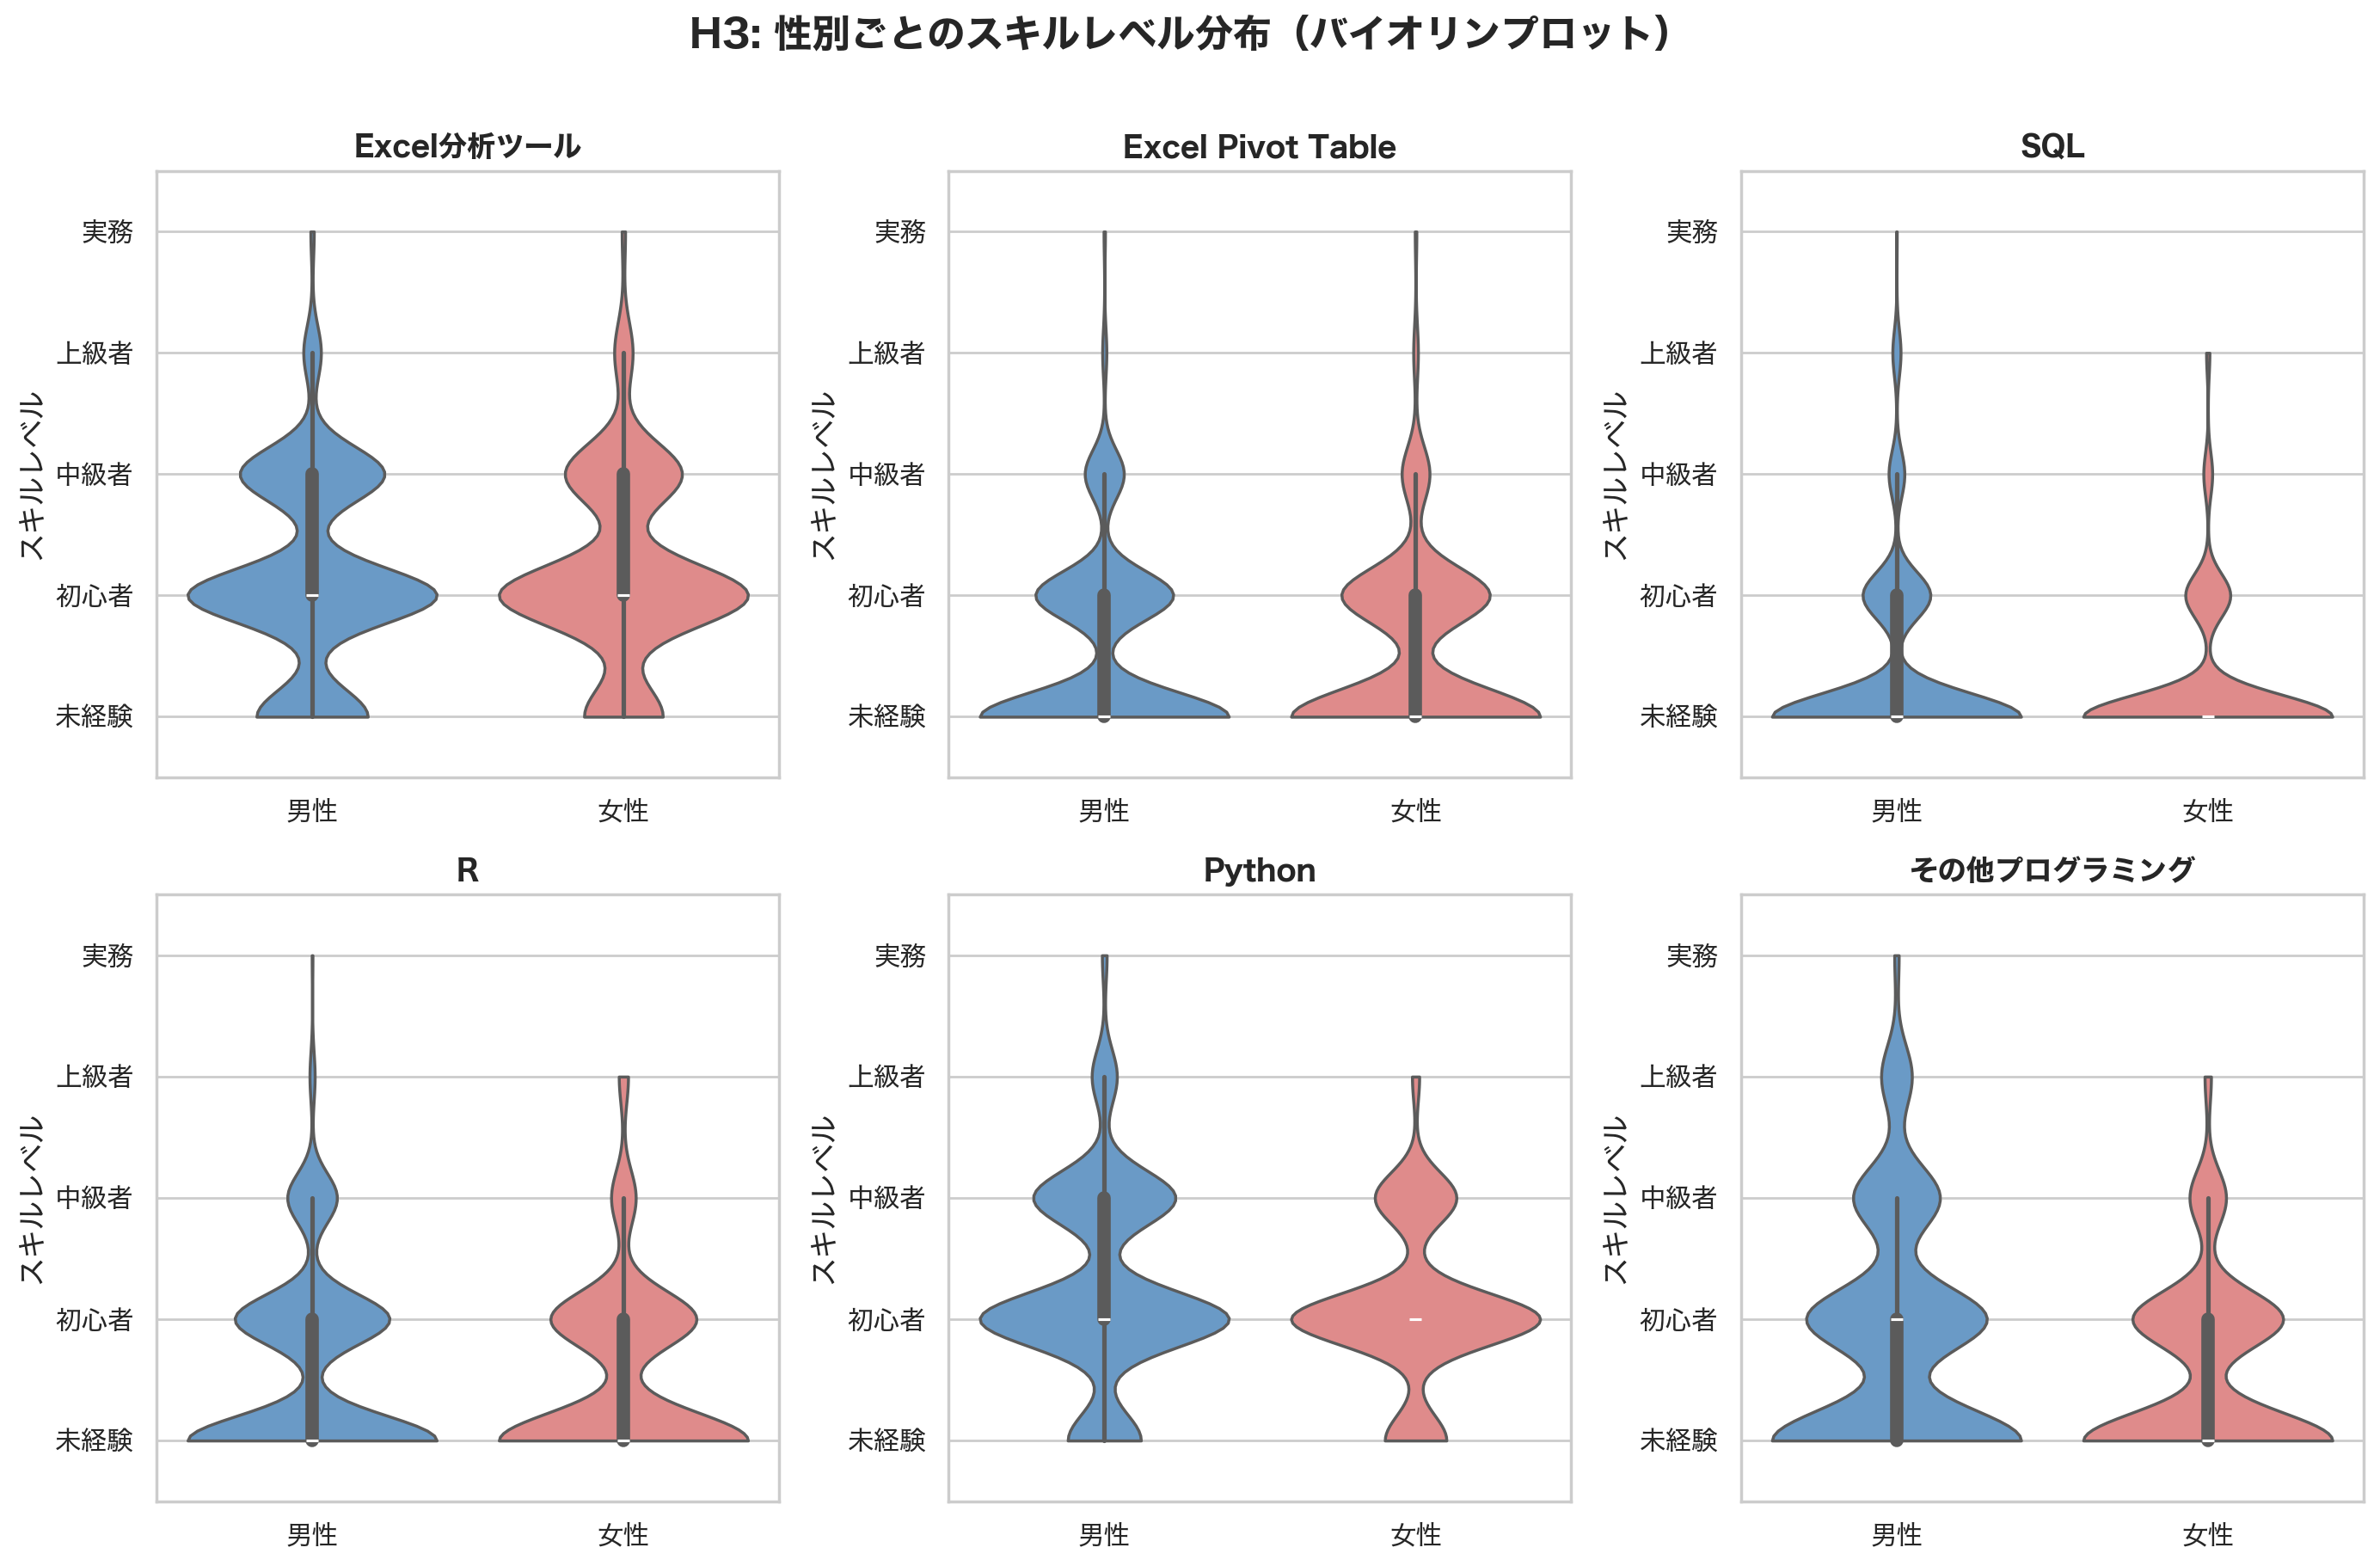
\includegraphics[width=0.52\linewidth]{../Assets/h3_gender_violin.png}
    \vspace{-3mm}
    \caption{H3: 性別ごとのスキル分布（Violin Plot）}
    \label{fig:h3_violin}
\end{figure}

% ============= PAGE 3: Micro Analysis (Math+Code) & Insights ==================
\newpage
\section{Pure NumPyによる相関係数の実装}
\label{sec:numpy_correlation}

ライブラリ依存ではない数学的理解の証明として，ピアソン相関係数をNumPyの基本演算のみで実装する\cite{numpy2020}．

\subsection{数学的背景 --- Covariance と Standard Deviation}

共分散（Covariance）$\mathrm{Cov}(X,Y)=\frac{1}{n}\sum(x_i\!-\!\bar{x})(y_i\!-\!\bar{y})$ と，
標準偏差（Standard Deviation）$\sigma_X=\sqrt{\frac{1}{n}\sum(x_i\!-\!\bar{x})^2}$ に対し，
ピアソン相関係数は共分散を両変数の標準偏差積で正規化（Normalization）した指標である：
%
\begin{equation}
    \rho_{X,Y}
    = \frac{\mathrm{Cov}(X,Y)}{\sigma_X \sigma_Y}
    = \frac{\displaystyle\sum_{i=1}^{n}(x_i - \bar{x})(y_i - \bar{y})}
    {\sqrt{\displaystyle\sum_{i=1}^{n}(x_i - \bar{x})^2
            \cdot \sum_{i=1}^{n}(y_i - \bar{y})^2}}
    \label{eq:pearson}
\end{equation}
%
$\bar{x},\bar{y}$は標本平均（Sample Mean）．計算は3段階に分解：
\textbf{(1)}~平均偏差 $d_{x_i}\!=\!x_i\!-\!\bar{x}$ （Mean Deviation），
\textbf{(2)}~共分散分子 $\sum d_{x_i}d_{y_i}$ （Covariance Numerator），
\textbf{(3)}~$L^2$ノルム正規化 $\rho = \mathrm{Cov}\big/\bigl(\lVert\bm{d}_x\rVert_2\!\cdot\!\lVert\bm{d}_y\rVert_2\bigr)$．

\subsection{実装コード}

\begin{lstlisting}[language=Python, caption={Pure NumPyによるピアソン相関係数}, label={lst:pearson}]
import numpy as np

def pearson_correlation(x: np.ndarray, y: np.ndarray) -> float:
    """Compute Pearson correlation coefficient using only NumPy primitives."""
    if len(x) != len(y):
        raise ValueError("Arrays must have equal length.")
    if len(x) < 2:
        raise ValueError("Need at least 2 data points.")

    # Step 1: Mean deviations  d_xi = xi - x_bar
    dx = x - np.mean(x)
    dy = y - np.mean(y)

    # Step 2: Covariance numerator = sum(dx * dy)
    numerator = np.sum(dx * dy)

    # Step 3: L2-norm normalization
    denominator = np.sqrt(np.sum(dx**2)) * np.sqrt(np.sum(dy**2))

    if denominator == 0.0:
        return 0.0  # Undefined (constant array)
    return float(numerator / denominator)
\end{lstlisting}

\vspace{-1mm}
\noindent\textbf{要点}：\texttt{np.mean}, \texttt{np.sum}, \texttt{np.sqrt}のみ使用し，\texttt{np.corrcoef}/\texttt{scipy.stats.pearsonr}への依存を排除．式\eqref{eq:pearson}の分子・分母を直接計算し，数式$\leftrightarrow$実装の1:1対応が検証可能．

\section{総合考察・提言と結論}

\vspace{-1mm}
\noindent\textbf{Actionable Insights}：
\textbf{(1)}~Python一強（$\bar{x}\!=\!2.22$/5），基礎復習は短縮可能．
\textbf{(2)}~SQL・R・Pivotは中央値1（未経験），ゼロからの導入が不可欠．
\textbf{(3)}~「Excel系」と「PG系」の2独立クラスターが存在（図\ref{fig:full_heatmap}）．
\textbf{(4)}~学部差は限定的（H2），学部混合で問題なし．
\textbf{(5)}~性別差は要配慮（H3），事前経験差であり能力差ではない．学部・性別混合ペアPG＋初学者スキャフォールディングを推奨．

\vspace{1mm}
\noindent\textbf{おわりに}：912名のアンケートから3仮説を検証し定量的講義設計提言を行った．
Python$\times$SQLの相関（$r\!=\!0.450$）はSFCのPG教育の相乗効果を示唆する．
今後は期末アンケートとの前後比較，クラスタリングによるセグメンテーション，成績予測力の評価を進める．

\vspace{-1mm}
\begin{thebibliography}{99}\footnotesize
    \bibitem{pearson1895} K. Pearson. Notes on Regression and Inheritance in the Case of Two Parents. \textit{Proc. R. Soc. Lond.}, 58:240--242, 1895.
    \bibitem{mann1947} H. B. Mann and D. R. Whitney. On a Test of Whether one of Two Random Variables is Stochastically Larger than the Other. \textit{Ann. Math. Statist.}, 18(1):50--60, 1947.
    \bibitem{numpy2020} C. R. Harris et al. Array programming with NumPy. \textit{Nature}, 585(7825):357--362, 2020.
\end{thebibliography}

\end{document}